\section{实验与结果分析}
在本章节中,我们评估了~\Mname{}在各种GNN模型和图数据集上的性能,对~\Mname{}的加速效果进行了全面的分析,并与现有的GNN框架(如DGL和PyG)进行了比较。我们还进行了一些附加实验研究,对GNN的隐藏维度,~\Mname{}的参数选择等问题进行了探讨。
\subsection{实验设置}
\hspace{5pt} \textbf{基准测试 (Benchmarks): }
我们选择了先前工作~\cite{wang2019dgl,pyG,ma2019neugraph} 在节点分类任务中广泛使用的两个最具代表性的 GNN 模型,以覆盖不同类型的聚合操作。
\underline{1) 图卷积网络 (GCN)}~\cite{GCNConv} 是最流行的 GNN 模型架构之一。
它也是许多其他 GNN(如图采样网络 GraphSAGE~\cite{SageConv} 和可微分池化 Diffpool~\cite{diffpool})的关键骨干网络。因此,提升 GCN 的性能也将惠及广泛的 GNN 模型。对于 GCN 的评估,我们采用以下设置:\textit{2 个层,隐藏维度为 16},这也是原始论文~\cite{GCNConv} 中的设置。
\underline{2) 图同构网络 (GIN)}~\cite{GINConv}。
GIN 与 GCN 的不同之处在于其聚合函数,该函数对节点自身的嵌入值进行加权。此外,GIN 也是许多其他具有更多边属性的更高级 GNN(如图注意力网络 GAT~\cite{GATConv})的参考架构。对于 GIN 的评估,我们采用以下设置:\textit{5 个层,隐藏维度为 64},这是原始论文~\cite{GINConv} 中使用的设置。

\textbf{基线 (Baselines): }
我们选择了两种同样基于 Pytorch 的图神经网络框架作为基线进行比较。
\underline{1) {Deep Graph Library (DGL})}~\cite{wang2019dgl} DGL 是一个专注于 GNN 计算效率的框架,特别是在 GPU 加速方面。它提供了针对多种主流 GNN 架构的高度优化的内核实现,并在许多标准图数据集和任务上展现出强大的性能。DGL 通过其底层的张量操作优化和高效的图表示,致力于为用户提供易于使用且性能卓越的 GNN 开发体验。
\underline{2) {Pytorch-Geometric (PyG})}~\cite{pyG} PyG 是另一个极其流行且功能强大的 GNN 框架,同样构建于 PyTorch 之上。PyG 以其灵活性和易于扩展性而闻名,尤其是在定义自定义 GNN 层和消息传递机制方面。它提供了一套简洁的 API,方便研究人员快速实现和迭代新颖的 GNN 模型。PyG 同样在性能方面表现出色,并在各种研究和应用中被广泛采用。

\textbf{数据集 (Datasets): }
我们涵盖了先前 GNN 相关工作~\cite{wang2019dgl, pyG, ma2019neugraph} 中使用的所有三种类型的数据集。
\underline{I 型图}是先前 GNN 算法论文~\cite{GCNConv, GINConv, SageConv} 常用的典型数据集。
它们的节点和边数量通常较小,但节点嵌入信息丰富且维度较高。
% These graphs can validate pure algorithm performance (\textit{e.g.}, the accuracy of link prediction).
% % 这些图可以验证纯粹的算法性能(例如,链接预测的准确性)。
\underline{II 型图}~\cite{KKMMN2016} 是图核 (graph kernels) 的流行基准数据集,并被选为 PyG~\cite{pyG} 的内置数据集。每个数据集包含一组小图,这些小图仅有图内边连接,没有图间边连接。
% These graphs are generally used for batched training or inference.
% % 这些图通常用于批量训练或推理。
\underline{III 型图} ~\cite{snapnets, GCNConv} 在节点和边的数量上都很大。这些图表现出高度的结构不规则性,这对大多数现有的 GNN 框架来说都具有挑战性。这些数据集的详细信息列于表~\ref{table: Evaluation Dataset}。
 % Note that $\#Class$ is used for node classification task.
其中,\textbf{\#类型}于节点分类任务。
\begin{table}[htbp] 
    \footnotesize % 使用较小的字体
    \caption{用于评估的数据集}
    \vspace{5pt} % 添加垂直空间,避免caption与表格重叠
    \centering
    \resizebox{0.9\textwidth}{!}{ % 使表格宽度与正文相同
        \begin{tabular}{|c|l|r|r|r|r|}
        \hline
        \textbf{类型} & \textbf{数据集} & \textbf{\#顶点} & \textbf{\#边} & \textbf{维度} & \textbf{\#类别} \\
        \hline
        \multirow{4}{*}{\textbf{I}} 
        & Citeseer    & 3,327	    & 9,464	    & 3,703 & 6      \\
        & Cora	    & 2,708     & 10,858	& 1,433 & 7      \\
        & Pubmed	    & 19,717	& 88,676	& 500  & 3      \\
        & PPI	        & 56,944	& 818,716	& 50   & 121    \\
        \hline
        
        \multirow{6}{*}{\textbf{II}}
        & PROTEINS\_full	&   43,471	       & 162,088	&   29	    & 2 \\
        & OVCAR-8H	    &   1,890,931	   & 3,946,402	&   66	    & 2 \\
        & Yeast	        &   1,714,644	   & 3,636,546	&   74	    & 2 \\
        & DD	            &   334,925	       & 1,686,092	&   89	    & 2 \\
        & TWITTER-Partial	&   580,768	       & 1,435,116	& 1,323    & 2 \\
        & SW-620H	        &   1,889,971	   & 3,944,206	&   66	    & 2 \\
        \hline
        
        \multirow{5}{*}{\textbf{III}} 
        & amazon0505	    & 410,236	& 4,878,875	    & 96  & 22 \\
        & artist	        & 50,515	& 1,638,396	    & 100 & 12 \\
        & com-amazon	    & 334,863	& 1,851,744	    & 96  & 22 \\
        & soc-BlogCatalog	& 88,784	& 2,093,195	    & 128 & 39 \\
        & amazon0601	    & 403,394	& 3,387,388	    & 96 & 22 \\
        \hline
        \end{tabular}
    }
    \vspace{-5pt}
    \label{table: Evaluation Dataset}
\end{table}


\textbf{平台与指标 (Platforms \& Metrics): }
\label{sect: Platforms and Metrics }
我们使用 CUDA 12.4 和 PyTorch 2.4.0 作为编程平台,基于 C++ 和 CUDA 实现了 ~\Mname{} 的后端,并通过 Python 绑定 PyTorch 前端。评估平台采用了一台配备 16 核心、32 线程的 AMD Ryzen 9 7945HX 处理器和 NVIDIA RTX 4060 GPU 的笔记本电脑,运行环境为 WSL2 下的 Ubuntu 24.04。在性能评估过程中,为了量化加速效果,我们通过计算 200 次端到端推理(前向传播)或训练(前向加反向传播)的平均延迟来衡量性能提升。
\subsection{性能评估}
在本节中,我们将详细展示~\Mname{}在GCN和GIN模型上的性能表现,并与DGL和PyG进行比较,涵盖训练和推理两个阶段。
\subsubsection{基于GCN的性能评估}
~\Mname{}在 GCN 上表现出色,在三种类型数据集上的训练和推理都实现了显著的加速效果。相比于 DGL, ~\Mname{}平均实现了$2.53 \times $的训练加速比和$3.13\times$的推理加速比;相比于PyG,~\Mname{}平均实现了$1.86\times$的训练加速比和$2.13\times$的推理加速比。接下来我们将详细分析~\Mname{}在 GCN 上的性能表现,并为每种数据集提供分析。
\begin{figure}[htbp] 
    \centering
    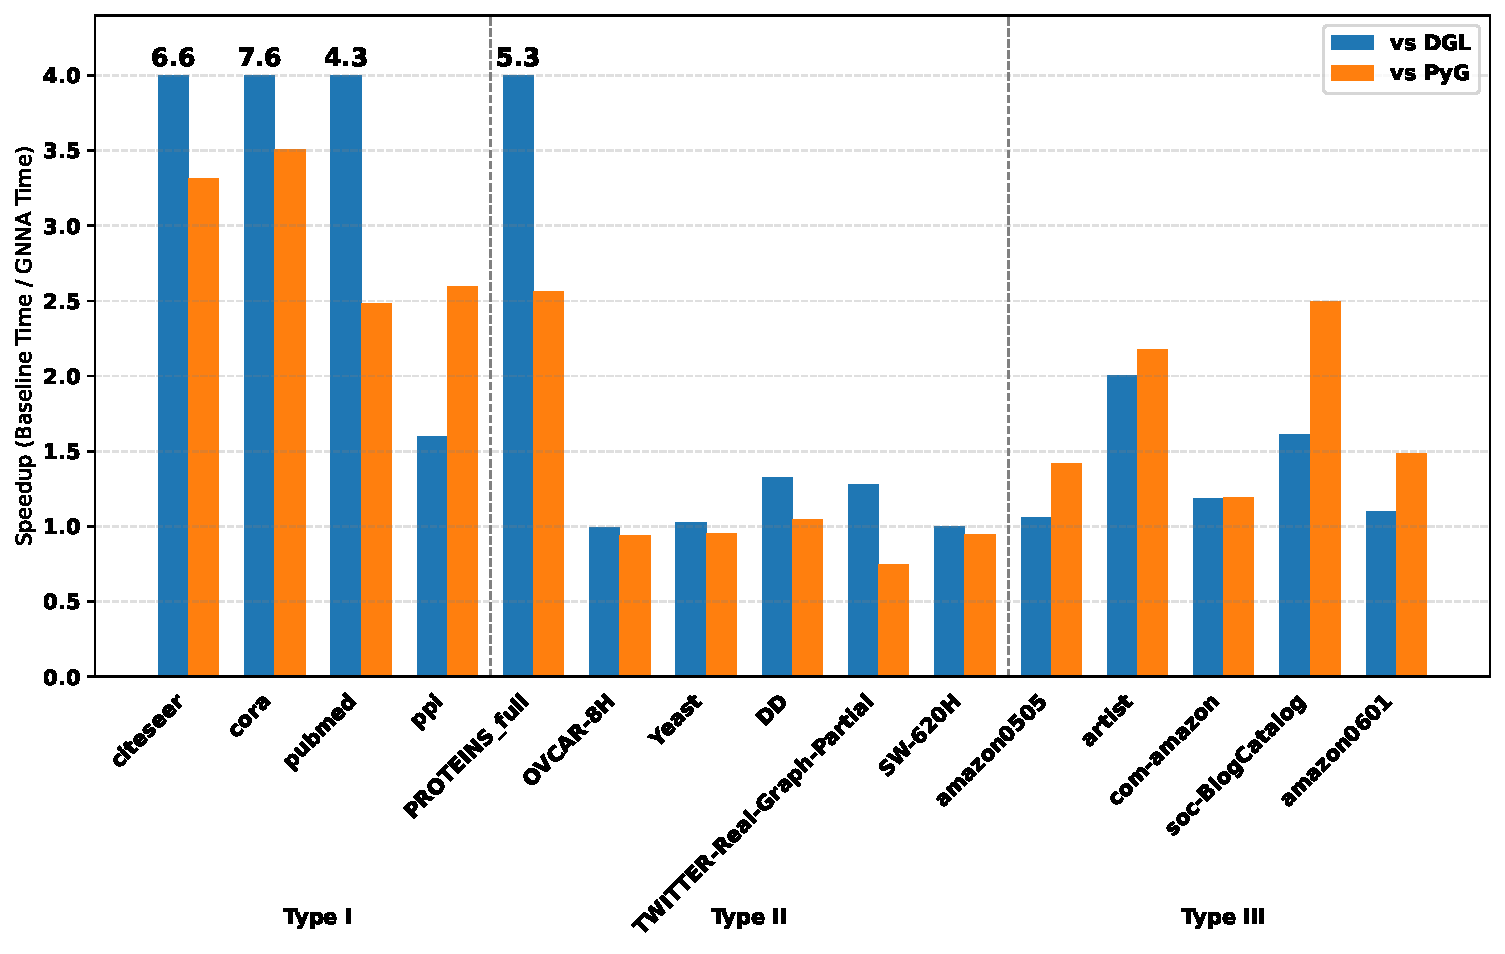
\includegraphics[width=\linewidth]{images/gcn_train_compare.pdf} 
    \caption{train speedup ($\times$) over DGL on GCN and GIN.}
    \label{fig: train-speedup-on-gcn}
    \setlength{\abovecaptionskip}{0.4cm} %增大caption和图像之间的距离
    \setlength{\belowcaptionskip}{-0.4cm} %缩小caption和下方文字的距离
\end{figure}

\textbf{I 型图:}
~\Mname{}在I型图上实现了最好的加速效果,相比于 DGL 取得了 $5.02\times$的训练加速比和$6.30\times$的推理加速比;相比于PyG取得了 $2.98\times$的训练加速比和$3.46\times$的推理加速比,在三种数据集中排第一位。I 型图的节点和边数量通常较小,但节点嵌入信息丰富且维度较高。~\Mname{}的按照维度划分工作线程的负载映射机制很好对此提供了很好的优化。

\textbf{II 型图:}
在此类数据集中,除了\textit{PROTEINS_full}外,~\Mname{}的性能要逊色于I型图。从训练的加速表现来看,加速比最高不超过$1.5\times$,在部分数据集上,表现不如PyG相对于 DGL 仅取得十分微弱的优势($1.02\times$);从推理的加速表现来看,相对于DGL取得了一定优势,平均推理加速比$2.36\times$,但是相比于PyG,推理加速效果较差,多个数据集中性能不及PyG。这是因为 II 型图的每个数据集包含一组小图,这些小图仅有图内边连接,没有图间边连接。PyG针对此类具有分块对角化邻接矩阵特性的批处理图数据优化最为全面(例如小批量处理机制),能够高效处理此类图结构数据。

\textbf{III 型图:}






\subsubsection{基于GIN的性能评估} 




\subsection{优化分析}
在这一节中,我们详细分析了~\ref{sect: design}中设计的优化策略。
\subsection{附加研究}

\subsection{本章小结}




% \subsection{与其他框架的比较}
% \subsubsection{与 DGL 的比较} \label{sect: compared with DGL}
% \begin{figure}[htbp] 
%     \centering
%     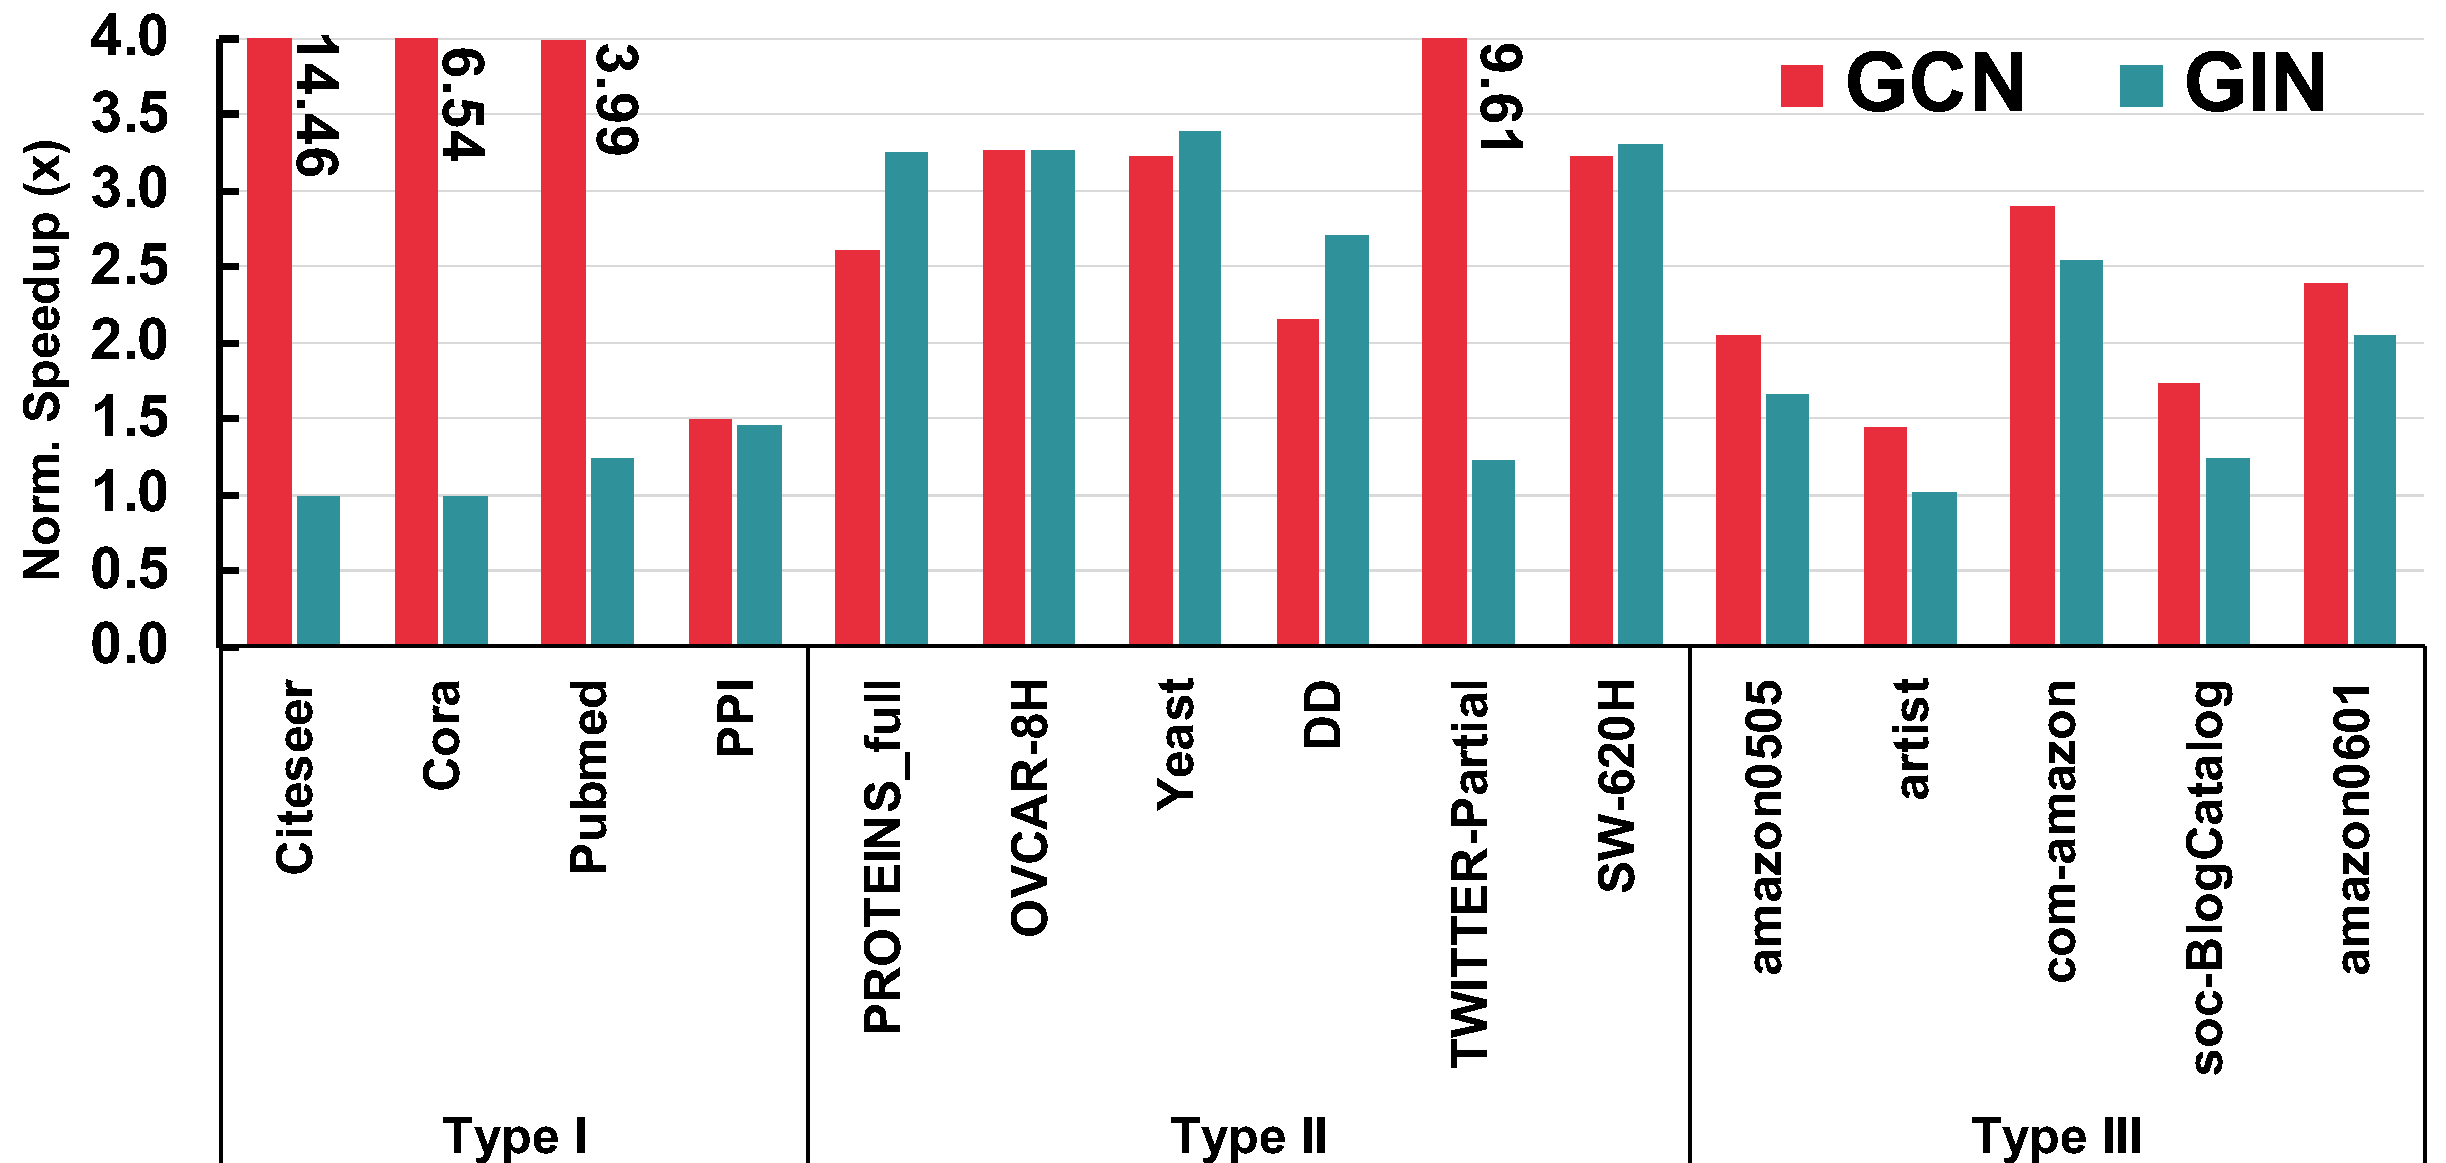
\includegraphics[width=0.9\linewidth]{images/dgl-speedup.pdf} 
%     \caption{Inference speedup ($\times$) over DGL on GCN and GIN.}
%     \label{fig: Speedup vs DGL.}
% \end{figure}
% 在本节中,我们首先在 GNN 推理方面与 DGL 进行了详细的实验分析和比较,然后将比较扩展到 GNN 训练。
% 如图~\ref{fig: Speedup vs DGL.} 所示,在 GCN 和 GIN 的推理任务上,针对三种类型的数据集,~\Mname{} 相较于 DGL~\cite{wang2019dgl} 分别平均取得了 todo 和 todo 的加速比。
% % Especially, on the challenging type III dataset, ~\Mname{}can still achieve an average $1.93\times$ speedup GCN and average $1.58\times$ speedup on GIN.
% % % 特别是,在具有挑战性的 III 型数据集上,\Mname 在 GCN 上仍能实现平均 1.93 倍的加速,在 GIN 上平均实现 1.58 倍的加速。
% % % It is because ~\Mname{}can fully leverage the input-level information, such as node degree, to guide system-level optimizations. %(\textit{e.g.}, group-based workload partitioning).  %thus maximizing the performance benefits on GPUs.
% % % % 这是因为 \Mname 可以充分利用输入层面的信息(例如节点度)来指导系统级优化(例如,基于组的工作负载划分),从而最大化 GPU 上的性能优势。
% % However, DGL only applies a set of generic optimizations without effectively using the input properties.
% % % % 然而,DGL 仅应用一组通用优化,而没有有效地利用输入属性。
% % We next provide detailed analysis for each type of datasets and give insights into the benefits based on low-level GPU kernel metrics.
% % % 我们接下来将对每种类型的数据集进行详细分析,并根据底层 GPU 核函数度量提供对其优势的见解。
% 接下来,我们将提供详细的分析,并针对每种类型的数据集给出见解。

% \textbf{I 型图:}
% 相较于 DGL,GCN 的性能提升(todo)显著高于 GIN(todo)。
% 主要原因是它们不同的 GNN 计算模式。
% 对于 GCN,节点维度缩减 (DGEMM) 总是在聚合操作之前进行。由于节点维度显著降低,这极大地减少了聚合阶段的数据移动和线程同步开销,
% %due to the significantly decreased node dimension, (原文注释:因为节点维度显著降低)
% 使得 GCN 可以从 ~\Mname{} 的二维工作负载管理和旨在改善数据局部性的专用内存优化中获得更多益处。另一方面,GIN 的聚合阶段必须节点维度缩减之前完成。因此,它无法避免在聚合阶段进行大量的内存访问和数据移动。因此,它从数据局部性以及用于快速且低开销内访问的 GPU 共享内存中获得的益处较少。然而,我们的细粒度维度划分仍然可以有效地处理这些高维情况。
% \begin{figure} [htbp]
%     \centering
%     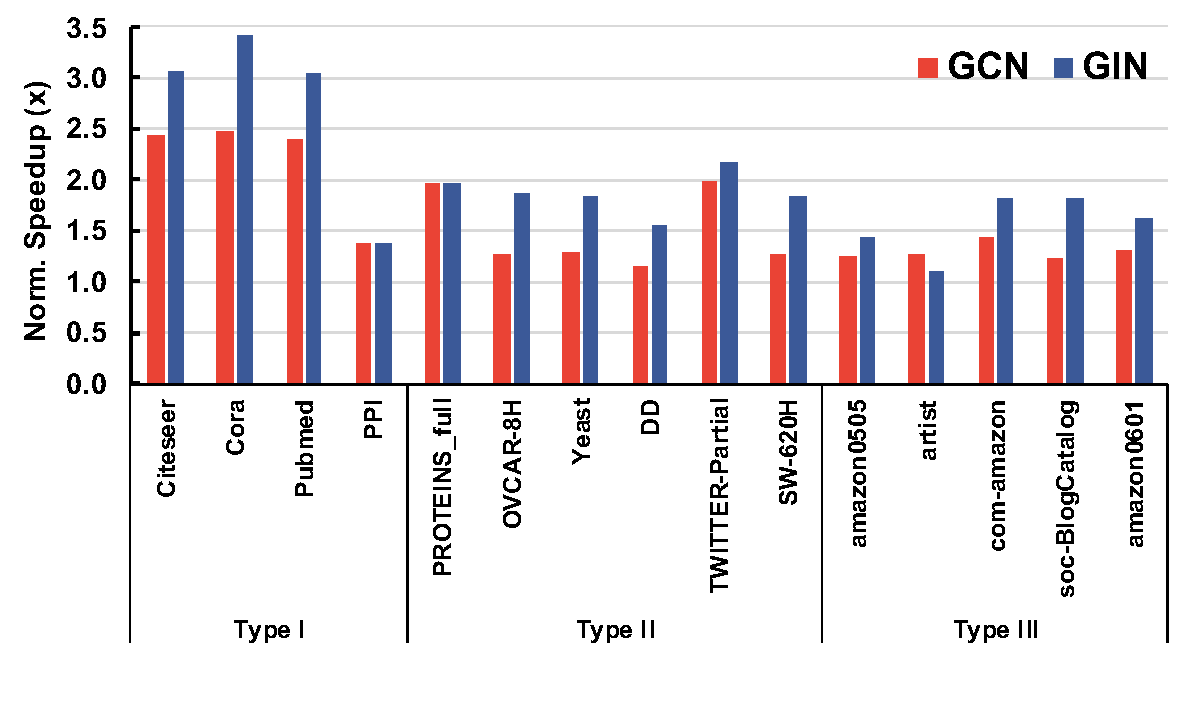
\includegraphics[width=0.9\linewidth]{images/GCN-training.pdf}
%     \caption{Training speedup ($\times$) over DGL on GCN and GIN.}
%     \label{fig: GCN Training Performance Comparison with DGL.}
% \end{figure}

% \textbf{II 型图:}
% 在相同数据集上,GCN (todo 倍) 和 GIN (todo 倍) 之间的性能差异相对较小,除了 \textit{TWITTER-Partial} 数据集,该数据集在类型二图中拥有最高的节点嵌入维度 (1323)。值得注意的是,与类型一图相比,GIN 的加速比始终更好。这主要有两个原因:1) 类型二图的节点特征维度(平均 66.5,不包括 \textit{TWITTER-Partial})远低于类型一图(平均 1421),这使得它们能从我们专用内存优化所带来的数据空间和时间局部性中获得更多性能益处;2) 类型二图本身在图结构上就具有良好的局部性。原因是类型二数据集由多个小图组成,这些小图内部连接非常密集,但图与图之间没有边连接,并且每个小图内的节点都被分配了连续的 ID。因此,当这种图结构局部性与 ~\Mname{} 高效的工作负载和内存优化相结合时,其带来的性能增益可以得到放大。

% \textbf{III 型图:}
% 在节点和边数量庞大的图(例如 \textit{amazon0505})上,加速比同样显著(GCN 平均 todo 倍,GIN 平均 todo 倍)。原因是高开销的线程间同步和全局内存访问可以通过我们的二维工作负载管理和专用内存优化得到很好的降低。
% % with significant performance tuning flexibility. % (原文注释:具有显著的性能调优灵活性。)
% 此外,我们的社区感知节点重编号通过改善数据的空间/时间局部性,进一步促进了相邻线程(处理一组节点)之间的高效工作负载共享。
% % In contrast, DGL only relies on simple and generic GPU kernel optimizations, while lacking an effective way to utilize the input-level information for performance improvement, thus suffering from inferior performance. % (原文注释:相比之下,DGL 仅依赖简单通用的 GPU 核函数优化,缺乏有效利用输入层信息来提升性能的方法,因此性能较差。)
% 在类型三中节点和边数量最少的数据集 \textit{artist} 上,我们注意到 GIN 的性能加速比较低。我们发现 \textit{artist} 数据集在类型三图中具有最高的图社区大小标准差,这使得以下两点变得具有挑战性:1) 利用组社区信息在 GNN 聚合阶段捕获节点的时空局部性,以及 2) 利用这种社区结构来指导系统级优化(例如,基于 Warp 的线程对齐和共享内存定制化)以在 GPU 上获取性能优势,因为 GPU 在每个块/SM 中具有固定数量的计算和内存单元。
% % in general. % (原文注释:通常而言。)

% \textbf{核函数度量 (Kernel Metrics):}
% 为了进行详细的核函数度量分析,我们利用 Nsight Compute~\cite{ncu} 来测量两个对性能至关重要的(计算和内存)CUDA 核函数度量指标:\textit{流式多处理器 (SM) 效率} 和 \textit{缓存 (L1 + L2 + 纹理) 命中率}。
% %
% 相较于 DGL,~\Mname{}在 GCN 和 GIN 上分别实现了平均 $todo$ 和 $todo$ 的更高 SM 效率,这表明我们的二维工作负载管理能够在单线程效率和多线程并行性之间取得良好平衡,这对整体性能提升至关重要。
% 相应地,相较于 DGL,~\Mname{}在 GCN 和 GIN 上分别实现了平均 $75.55\%$ 和 $126.20\%$ 的更高缓存命中率,这展示了专用内存优化的好处。

% \vspace{-10pt}
% \textbf{训练支持 (Training Support):}
% 我们还在所有三种类型的数据集上评估了 ~\Mname{} 相对于 DGL 在 GCN 和 GIN 上的训练性能。
% 与推理相比,训练更具挑战性,因为它涉及更密集的计算,包括前向值传播和反向梯度传播,这两者都严重依赖于底层的图聚合核函数进行计算。
% 如图~\ref{fig: GCN Training Performance Comparison with DGL.}所示,~\Mname{} 始终优于 DGL 框架,在 GCN 和 GIN 上分别取得了平均 todo 和平均 todo 的加速比,这显示了我们输入驱动优化的优势。
% % \todo{Q: Less training speedup:} % 问题:为何训练加速比较低?
% % \fixed{
% GNN 训练与推理的关键区别有两方面:首先,训练需要反向传播。这一步受益于我们的改进,因为反向传播步骤与推理期间的前向计算类似,所有提出的方法仍然有益;其次,训练会产生额外的内存和数据移动开销,用于存储/访问前向传播的激活值,直到梯度可以反向传播回来。
% % This is the reason for lower training speedup. % 这就是训练加速比较低的原因。
% % In contrast, in the inference, all such intermediate results can be thrown away immediately when the computation processes to the next layer. % 相比之下,在推理中,当计算进行到下一层时,所有这些中间结果都可以立即丢弃。
% % }

% \subsubsection{与 PyG 的比较}
% % We choose the best setting of PyG: Type II datasets + graph mini-batching. Other settings are omitted due to inferior results. % 我们选择 PyG 的最佳设置:类型二数据集 + 图小批量处理。其他设置因结果较差而被省略。
% % the comparison with PyG in end-to-end training since PyG has the most optimizations (\textit{e.g.}, ) for effectively processing such batched graphs with block-diagonal properties in their adjacent matrices. % 在端到端训练中与 PyG 进行比较,因为 PyG 具有最多的优化(例如,...)来有效处理邻接矩阵具有块对角属性的批处理图。
% % For Type I and III datasets, we find that PyG cannot provide comparable performance compared with DGL and thus decide not to include the results here. % 对于类型一和类型三数据集,我们发现 PyG 无法提供与 DGL 相当的性能,因此决定不在此处包含结果。
% 如图~\ref{fig: Comparison with PyG.}所示,~\Mname{}的表现优于 PyG,在 GCN 和 GIN 上分别取得了平均 $todo$ 和 $todo$ 的加速比。对于 GCN,~\Mname{}在具有高维节点嵌入的数据集(例如 \textit{TWITTER-Partial})上实现了显著的加速,这得益于:1) 在聚合前进行节点维度缩减;以及 2) 通过邻居划分和维度划分实现工作负载共享。对于 GIN,~\Mname{}在平均度较高的数据集(例如 \textit{DD})上达到了 $todo$ 的加速比,因为 ~\Mname{}能够有效地将每个节点的工作负载沿着其嵌入维度分发给工作线程,同时兼顾了单线程效率和线程间并行性。相比之下,PyG 的性能较差,原因在于:1) 其在平衡工作负载和控制同步开销方面的线程管理策略效率不高;2) 它严重依赖灵活性不足的 scatter-and-gather 核函数。
% \begin{figure}[t]
%     \centering
%     % \vspace{-5pt}
%     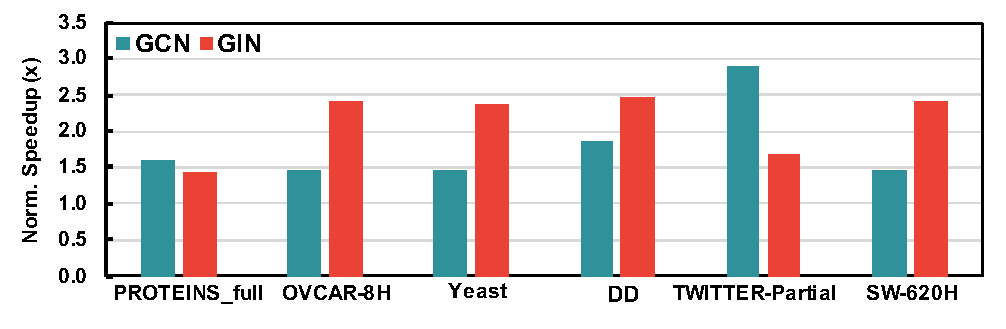
\includegraphics[width=0.9\linewidth]{images/pyg-gcn-gin.pdf}
%     \caption{在 GCN 和 GIN 上相对于 PyG 的训练加速比 ($\times$)。}
%     \label{fig: Comparison with PyG.}
% \end{figure}

% \subsection{优化分析}
% \label{sect: Optimization Analysis}
% % \vspace{-5pt}
% 在本节中,我们详细探讨并分析第~\ref{sect: 2D Workload Management}节和第~\ref{sect: Specialized Memory Optimization}节中使用的优化方法。
% % the advantage of 2D workload of ~\Mname{}by exploring the impact of \textit{neighbor-group}, \textit{thread-per-block}, and \textit{dimension-worker} on GCN performance.
% % % 通过探索邻居组、每块线程数和维度工作线程对 GCN 性能的影响,来探讨 \Mname 的二维工作负载的优势。
% % compute efficiency (SM efficiency + atomic transactions), and memory performance (cache hit ratio, and memory throughput)
% % % 计算效率(SM 效率 + 原子事务)和内存性能(缓存命中率、内存吞吐量)
% % \begin{figure} [h] \small
% %     \centering
% %     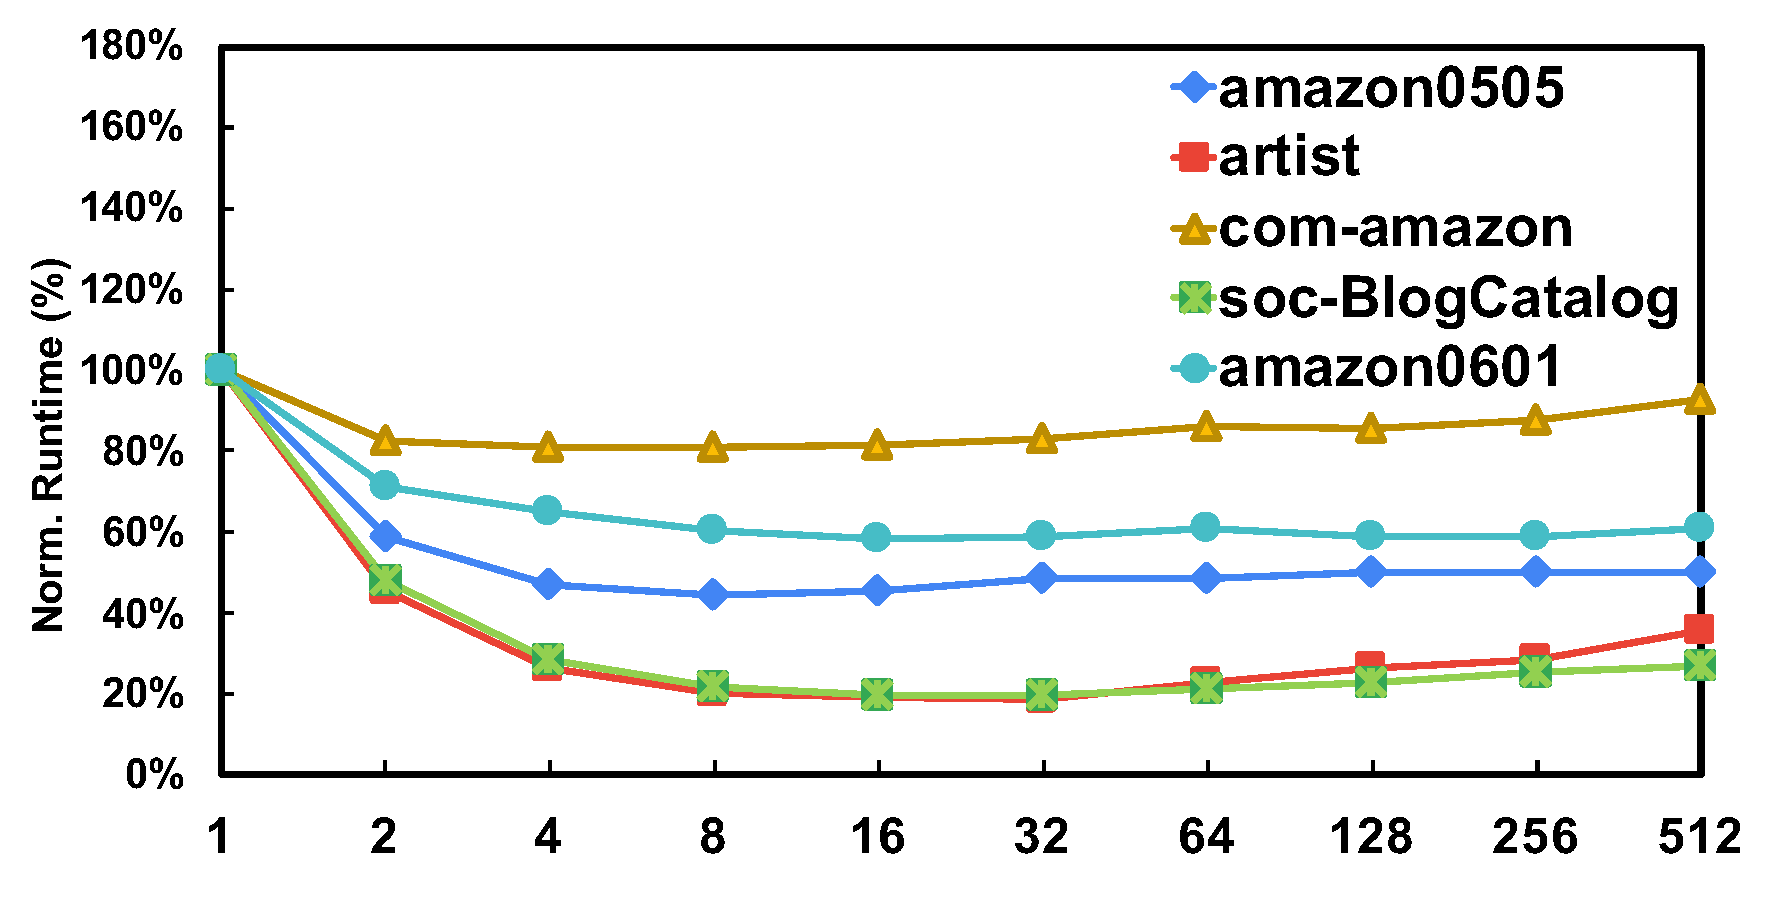
\includegraphics[width=0.9\columnwidth]{imgs/group-size-study.pdf}
% %     \caption{Group Size Impact. \small{Note: we normalize the runtime of other group size settings \textit{w.r.t.} the group size=1 setting ($100\%$).}}
% %     % % 组大小的影响。注:我们将其他组大小设置的运行时相对于组大小=1的设置进行了归一化(100%)。
% %     \vspace{-10pt}
% %     \label{fig: Group-size Vs. Performance.}
% % \end{figure}

% % \begin{figure*}[h] \small
% %     \centering
% %     \subfloat[]{\includegraphics[width=0.33\textwidth]{imgs/node-reordering-speedup.pdf}}
% %     \subfloat[]{\includegraphics[width=0.5\textwidth, trim=0 -0.5cm 0 0 ]{imgs/node-reordering-metrics.pdf}}
% %     \subfloat[]{\includegraphics[width=0.33\textwidth, trim=1cm 1.2cm 0 1cm]{imgs/block-based-memory.pdf}}
% %     % \vspace{-10pt}
% %     \caption{Group-based Workload Impact on Performance (a) Group Size, (b) Thread-per-block, and (c) Dimension worker.}
% %     % % 基于组的工作负载对性能的影响 (a) 组大小,(b) 每块线程数,(c) 维度工作线程。
% %     % \vspace{-12pt}
% %     \label{fig: Detailed GPU Metrics Comparison with DGL.}
% % \end{figure*}

% %\noindent
% % \vspace{1pt}
% \textbf{邻居划分 (Neighbor partitioning):}
% 从图todo可以看出,随着邻居组大小的增加,~\Mname{}的运行时间会先下降。邻居组大小的增加可以充分利用每个线程的计算能力,同时提高了数据局部性并减少了原子操作的数量(即线程间同步开销)。然而,当邻居组大小超过某个阈值(例如,对于 \textit{artist} 数据集是 32)时,每个线程达到了其计算能力的上限,进一步增加邻居组大小不再带来性能提升,反而会增加整体延迟。

% \textbf{维度划分 (Dimension partitioning):}
% 如图todo所示,与邻居组大小相比,维度工作线程数量在 1 到 16 的范围内对性能的影响更为明显。
% 当维度工作线程数量从 16 增加到 32 时,由于单工作线程效率和多工作线程并行性已经达到平衡,运行时间性能差异非常小。因此,进一步增加维度工作线程数量不再带来更多好处。
% % of Type III datasets could reach its optimal, which can balance the single-worker efficiency and the multi-worker parallelism. % (原文片段:类型三数据集可以达到其最优值,这可以平衡单工作线程效率和多工作线程并行性。)
% % The even larger size of dimension worker lets some launched threads get fewer dimensions to work on. % (原文片段:更大的维度工作线程数量让一些启动的线程分配到更少的维度进行工作。)
% % The overall performance decreases due to the thread under-utilization. % (原文片段:由于线程利用率不足,整体性能下降。)
% \begin{figure}[htbp] \small
%     \vspace{-8pt}
%     \subfloat[]{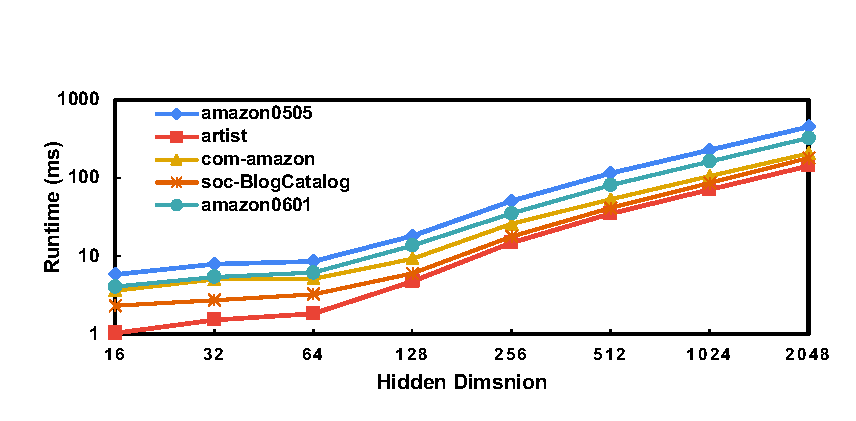
\includegraphics[width=0.48\linewidth, height=2.4cm, trim=0 0.3cm 0 0]{images/dimension-gcn.pdf}} 
%     \hfill % 添加水平间距
%     \subfloat[]{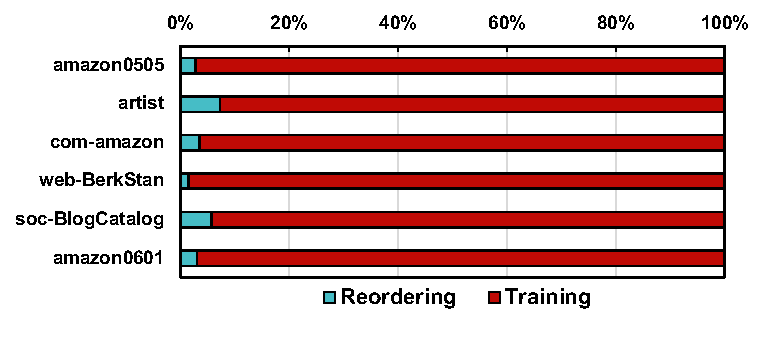
\includegraphics[width=0.48\linewidth, height=2.4cm, trim=0 -0.1cm 0 -0.1cm]{images/reordering-overhead.pdf}} 
%     \vspace{-10pt}
%     \caption{(a) Dimension comparison for GCN; (b) Reordering overhead.}
%     \label{fig: Additional Studies.}
% \end{figure}



% \textbf{节点重编号 (Node renumbering):}
% 我们通过对类型三数据集上的 GCN 和 GIN 进行性能剖析,展示了节点重编号的好处。如图todo所示,对图中的节点进行重编号可以分别为 GCN 和 GIN 带来高达 $todo$ 和 $todo$ 的加速比。主要原因是我们的社区感知节点重编号能够增加 GNN 聚合过程中的数据空间和时间局部性。

% 为了量化这种局部性带来的好处,我们提取了详细的 GPU 核函数度量指标——以从 DRAM 读取和写入的字节数表示的内存访问量,来进行说明。
% 我们的 CUDA 核函数度量剖析结果显示,节点重编号可以有效地减少运行时的内存访问开销(GCN 平均减少 todo\%,GIN 平均减少 todo\%),因为更多加载的节点嵌入更有可能在具有连续 ID 的节点之间共享。
% 我们也注意到一个从我们的优化中受益较少的输入案例——\textit{artist},因为:1) \textit{artist} 内部的社区大小呈现出很大的变异性(标准差高),这使得捕获邻接关系和局部性变得困难;2) 这种变异性阻碍了系统级(计算和内存)优化有效地利用重编号带来的局部性优势。

% \textbf{块级优化 (Block-level optimization):}
% 我们展示了我们的块级优化(包括基于 Warp 的线程对齐和 Warp 感知的共享内存定制化)带来的优化效益。
% 我们分析了两个核函数度量(\textit{原子操作减少量}和\textit{DRAM 访问减少量})在三个大图上的情况作为示例。
% 如图 todo 所示,~\Mname{}可以有效地将原子操作和 DRAM 内存访问分别平均减少 todo 和 todo。
% 这个结果表明:
% 1) 基于邻居划分的 Warp 对齐线程映射能够有效减少大部分原子操作;
% 2) Warp 感知的共享内存定制化能够避免大量的全局内存访问。

% \vspace{-6pt}
% \subsection{附加研究}
% \label{sect: Additional Studies}
% \hspace{5pt} \textbf{GNN 的隐藏维度 (Hidden dimensions of GNN):}
% 在本实验中,我们分析了 GNN 架构中隐藏维度大小对 GCN 和 GIN 的影响。
% 如图todo 所示,我们观察到随着 GCN 隐藏维度的增加,~\Mname{}的运行时间也随之增加,这是因为聚合阶段需要更多的计算(例如,加法)和内存操作(例如,数据移动),以及节点更新阶段节点嵌入矩阵的尺寸更大。
% 同时,我们也注意到 GIN 相对于 GCN 显示出更大的延迟增长,这主要是因为层数不同(2 层 GCN 对比 5 层 GIN)使得这种差异更加显著。

% \textbf{开销分析 (Overhead analysis):}
% 社区感知节点重编号是利用 GNN 输入信息产生开销的主要来源,其他部分的开销可以忽略不计。
% 这里作为一个案例研究,我们根据 ~\Mname{}\textbf{Decider} 给出的优化决策(如第~\ref{sect: Specialized Memory Optimization}节所讨论),评估了它在类型三图上 GCN 训练阶段的开销。
% 这里我们使用训练作为示例;在真实的 GNN 应用场景中,推理过程也会使用相同的图结构很多次~\cite{SageConv, GCNConv, GCNConv},只是输入不同的节点嵌入。
% 如图todo所示,与整体训练时间相比,节点重编号的开销始终很小(平均 4.00\%)。
% % TODO in GNN both training and inference would use the same graph structure many times~\cite{SageConv, GCNConv, GCNConv} while only changing the node embeddings input, therefore, we use training for illustration. % (原文注释:注意,在 GNN 中,训练和推理都会多次使用相同的图结构,仅改变节点嵌入输入,因此我们使用训练作为示例。)
% 因此我们得出结论,这种一次性开销可以在 GNN 的运行时间内被分摊,这证明了它在实际 GNN 应用中的适用性。

% \begin{figure} [t] \small
%     \centering
%     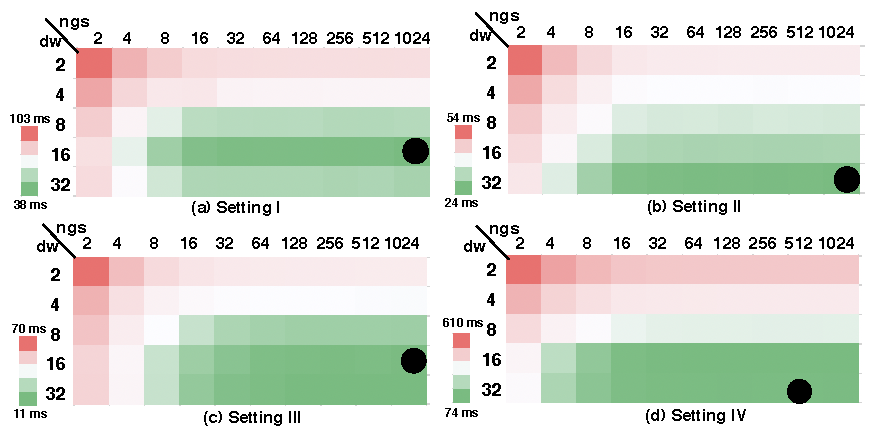
\includegraphics[width=\columnwidth]{images/analytical-modeling-1.pdf}
%     \vspace{-10pt}
%     \caption{四种设置的参数选择。注意,黑色实心点表示由 ~\Mname{}\textbf{Decider} 基于分析模型选择的参数 ($\mathit{dw}$ 和 $\mathit{ngs}$)。}
%     \vspace{-15pt}
%     \label{fig: Parameter Selection for Four Settings}
% \end{figure}

% \textbf{参数选择 (Parameter selection):}
% 为了展示我们分析模型在核函数参数选择方面的有效性,我们考虑了四种不同的设置:
% I: 以 \textit{amazon0505} 在 P6000 GPU 上的 GCN 作为我们的基准设置;
% II: \textit{amazon0505} GCN 在 V100 上,以展示设备适应性;
% III: \textit{amazon0505} 和 \textit{soc-BlogCatalog} 在 P6000 上,以展示对不同数据集的适应性;
% IV: \textit{amazon0505} 在 P6000 上的 GIN,以展示对不同 GNN 模型架构的适应性。
% 如图~\ref{fig: Parameter Selection for Four Settings}所示,我们的参数选择策略能够为上述四种设置精确地找到最优的低延迟设计。
% 这证明了我们的分析模型在辅助参数选择以优化 GNN 计算性能方面的有效性。
